\documentclass{article}

% --- NeurIPS 2025 style (submission mode — anonymous, with line numbers) ---
\usepackage{neurips_2025}

\usepackage[utf8]{inputenc}
\usepackage[T1]{fontenc}
\usepackage{hyperref}
\usepackage{url}
\usepackage{booktabs}
\usepackage{amsfonts}
\usepackage{nicefrac}
\usepackage{microtype}
\usepackage{graphicx}

% ============================================================
\title{Agentic Expense Claims: A Multi-Agent Multimodal System \\
for Automated Expense Report Processing}
% ============================================================

% --- Authors (hidden in submission mode; shown in final) ---
\author{%
  Author 1 \\
  \texttt{author1@sutd.edu.sg} \\
  \And
  Author 2 \\
  \texttt{author2@sutd.edu.sg} \\
  \And
  Author 3 \\
  \texttt{author3@sutd.edu.sg} \\
  \And
  Author 4 \\
  \texttt{author4@sutd.edu.sg} \\
}

\begin{document}

\maketitle

% ============================================================
\begin{abstract}
% [TODO] ~150 words. Summarize:
% - Problem: expense claims are manual, error-prone, multi-modal
% - Approach: 4-agent system (Intake, Compliance, Fraud, Advisor)
%   orchestrated by LangGraph, grounded in receipt images + policy text + structured DB
% - Key contribution: agentic redesign that eliminates manual data entry,
%   prevents policy violations pre-submission, and auto-approves low-risk claims
% - Preliminary results / evaluation plan
\end{abstract}

% ============================================================
\section{Problem Decomposition}
\label{sec:problem}
% ============================================================

\subsection{Problem Statement}
\label{sec:problem-statement}

% [TODO] Define the expense claims problem.
% - Current process: form-based, manual data entry, multi-level approval
% - Context: SUTD SAP Concur system
% - Core argument: why this cannot be solved by a single model call
%   (multiple reasoning stages, multiple modalities, multiple stakeholders)

\subsection{Current Workflow Pain Points}
\label{sec:pain-points}

% [TODO] Empirically observed pain points from SUTD SAP Concur analysis:
%
% \begin{enumerate}
%   \item High error rates in OCR-based receipt scanning
%   \item Lengthy submission times (15--25 min per claim)
%   \item Policy confusion across 5 claim policies and 20+ GL codes
%   \item Repeated claim rejections (missing/incorrect fields)
%   \item Multi-modal complexity (receipts, PDFs, itineraries, policy text)
%   \item No automated validation or intelligent suggestions
% \end{enumerate}

\subsection{Sub-Task Decomposition}
\label{sec:subtasks}

% [TODO] Explicit decomposition into distinct reasoning/decision-making stages.
% Must have >= 3 stages that cannot be merged into a single model invocation.
%
% Stage 1: Multimodal data extraction (receipt images -> structured data via VLM)
% Stage 2: Policy compliance validation (pre-submission evaluator-optimizer loop)
% Stage 3: Post-submission parallel assessment (compliance audit + fraud investigation)
% Stage 4: Risk-based routing and advisory (risk scoring + human-assisted review)
%
% Argue why merging these into one prompt is infeasible:
% - Different modalities at each stage
% - Different tools required
% - Independent concerns (compliance vs fraud)
% - Human-in-the-loop at review stage

% ============================================================
\section{Agent Architecture}
\label{sec:architecture}
% ============================================================

\subsection{System Diagram}
\label{sec:system-diagram}

% [TODO] Insert system architecture figure showing:
% - Entry point (role-based routing)
% - Intake Agent -> Compliance Agent + Fraud Agent (parallel) -> Advisor Agent
% - MCP server connections
% - User interfaces (Claimant chat, Reviewer inbox)
%
% \begin{figure}[h]
%   \centering
%   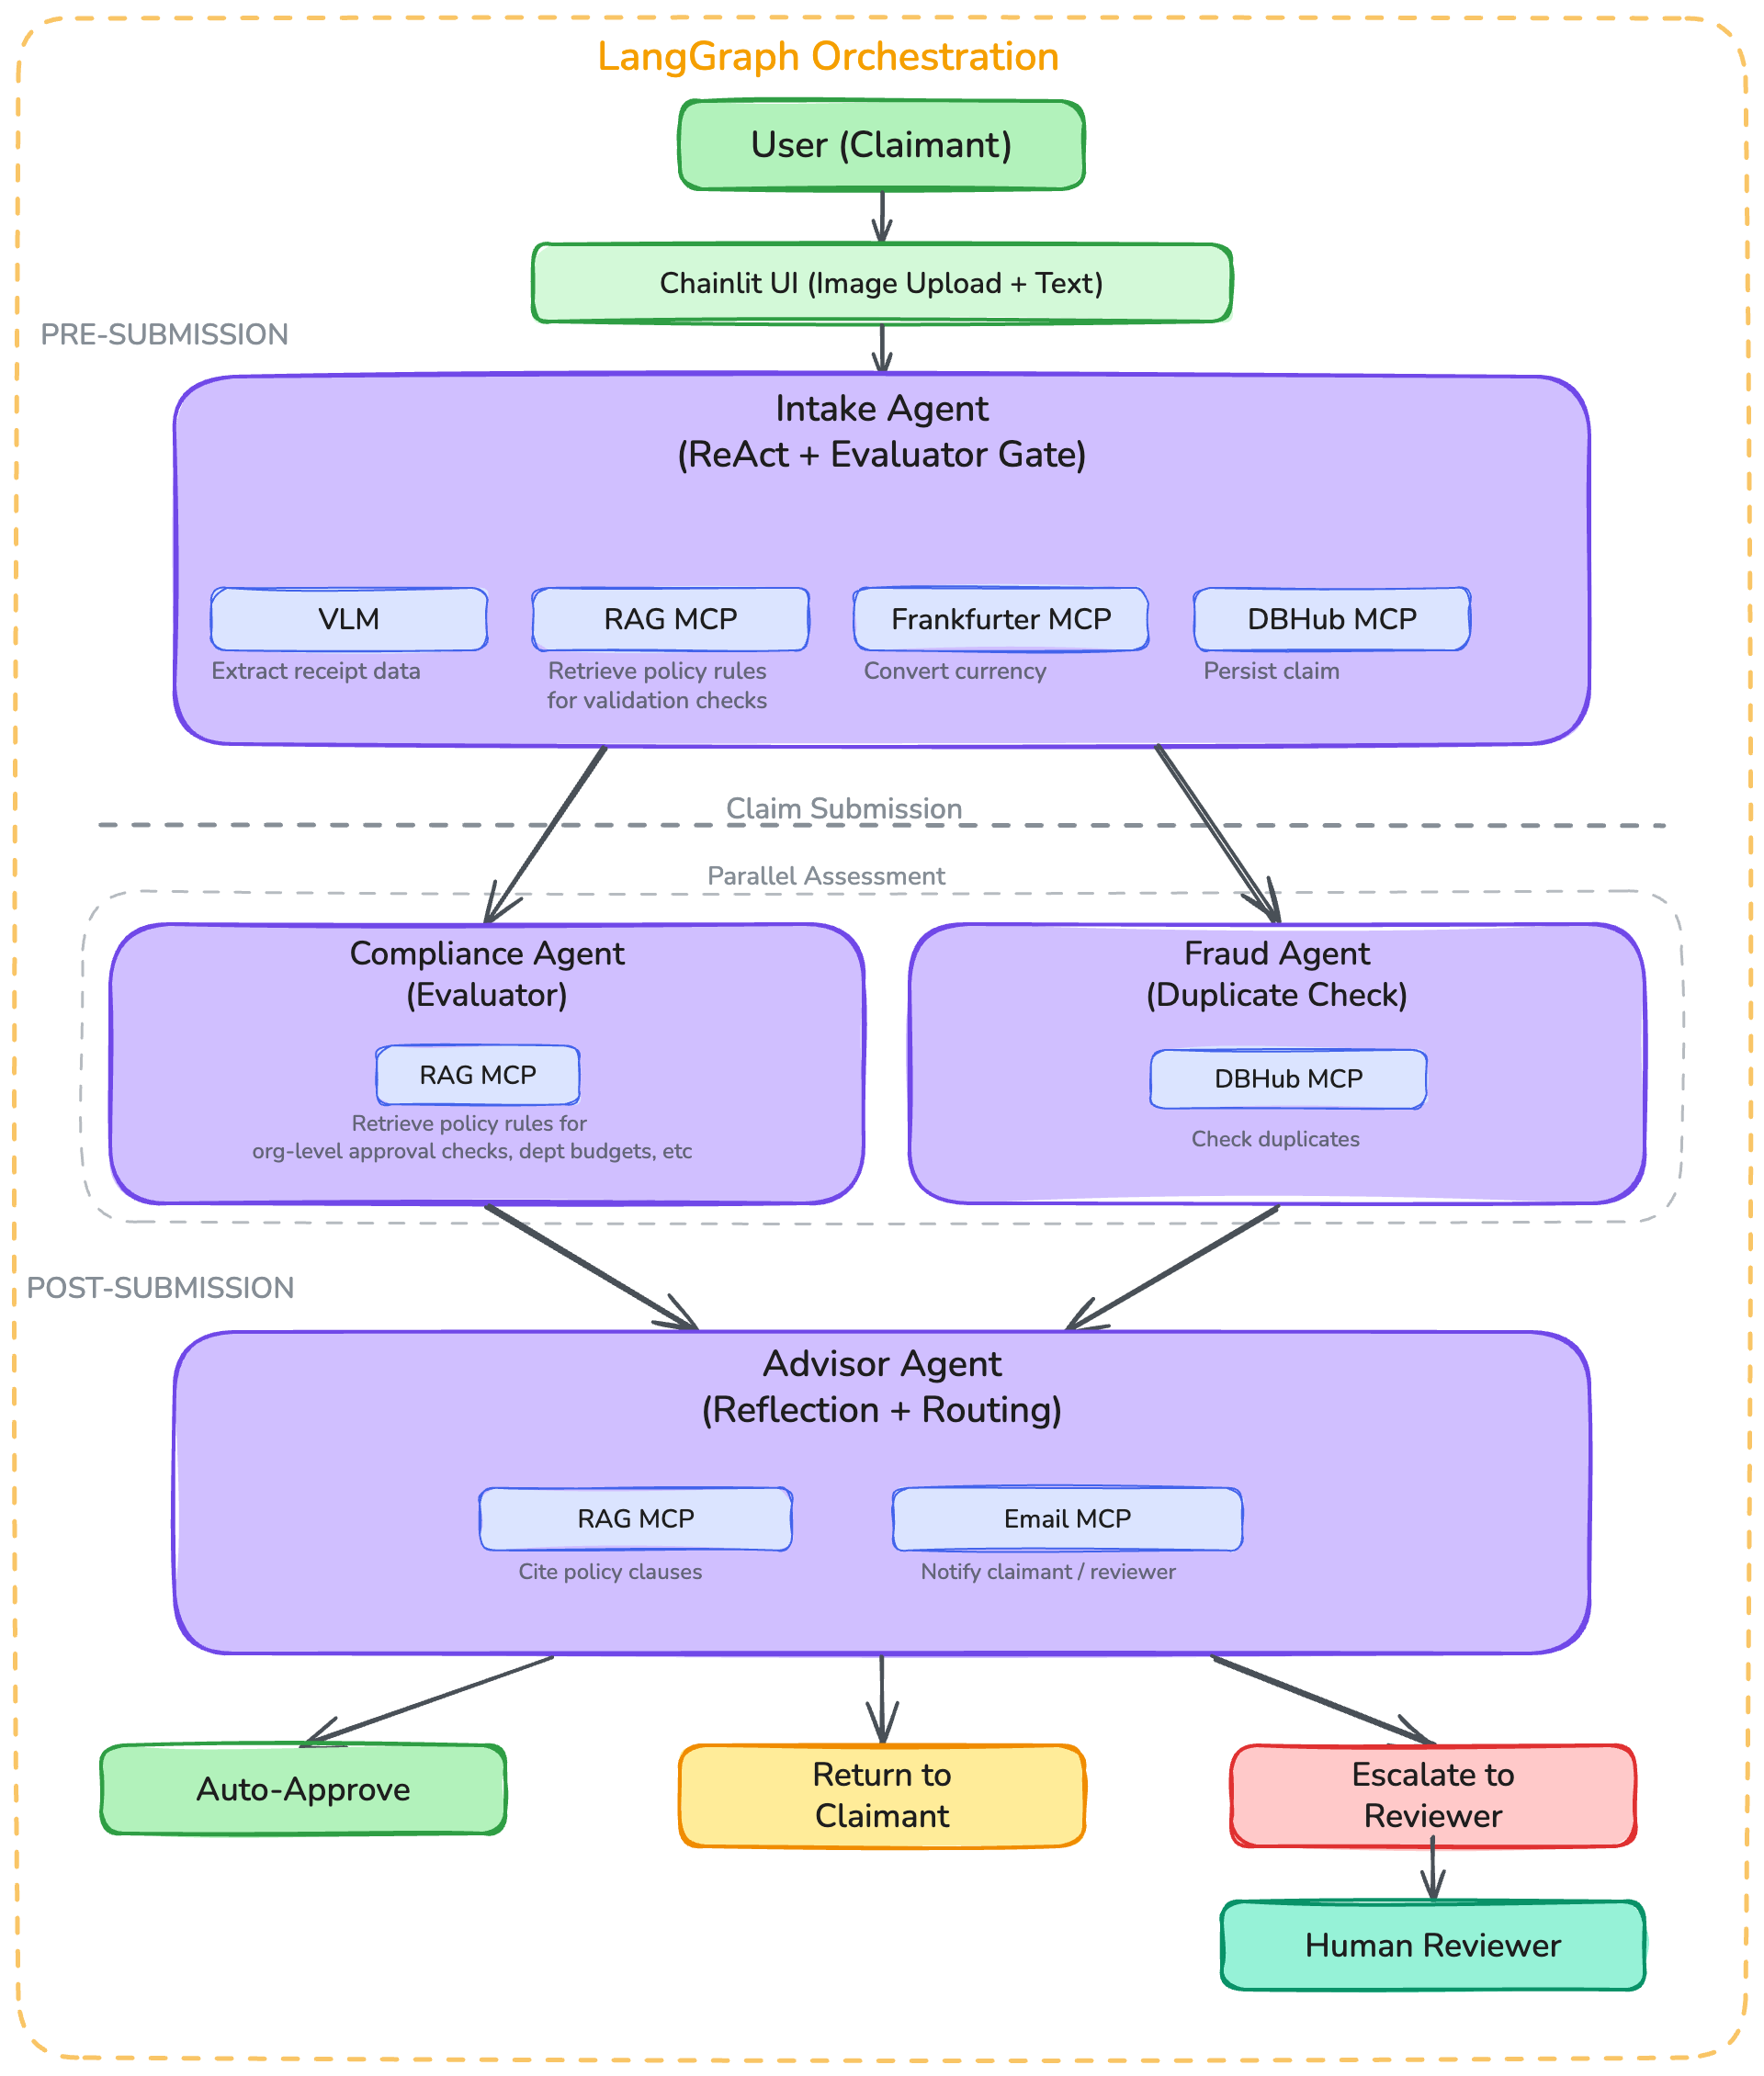
\includegraphics[width=\textwidth]{figures/system-architecture.pdf}
%   \caption{System architecture of the agentic expense claims pipeline.}
%   \label{fig:architecture}
% \end{figure}

\subsection{Agent Roles}
\label{sec:agent-roles}

% [TODO] Define each agent. Use table below as starting point.
%
% \begin{table}[h]
%   \centering
%   \caption{Agent definitions and agentic design patterns.}
%   \label{tab:agents}
%   \begin{tabular}{@{}llll@{}}
%     \toprule
%     Agent & Pattern & Serves & Responsibility \\
%     \midrule
%     Intake Agent      & ReAct + Evaluator-Optimizer & Claimant & [TODO] \\
%     Compliance Agent  & Evaluator-Optimizer         & System   & [TODO] \\
%     Fraud Agent       & Prompt Chaining             & System   & [TODO] \\
%     Advisor Agent     & Reflection + Routing        & Reviewer & [TODO] \\
%     \bottomrule
%   \end{tabular}
% \end{table}

\subsection{Model and Tool Choices}
\label{sec:model-tools}

% [TODO] Justify selection of:
% - Orchestration: LangGraph (deterministic graph + LLM-powered nodes)
% - VLM for receipt extraction (model TBD — e.g., GPT-4o, Gemini, Qwen-VL)
% - LLM for reasoning agents (model TBD)
% - MCP servers: DBHub (Postgres), rag-mcp-server (policy RAG),
%   Frankfurter (currency), Forensics-MCP-Server (receipt image forensics),
%   mcp-email-server (notifications)

\subsection{User Interface}
\label{sec:ui}

% [TODO] Describe the usable UI for demo:
% - Chainlit chat interface
% - Two personas: Claimant (submit claims via conversation) and Reviewer (review queue)
% - Receipt upload via drag-and-drop
% - Include a UI mockup or screenshot if available

% ============================================================
\section{Multimodal Grounding}
\label{sec:multimodal}
% ============================================================

\subsection{Modalities Used}
\label{sec:modalities}

% [TODO] At least two modalities. This system uses three:
%
% 1. Image: Receipt photos, scanned documents (processed by VLM)
% 2. Text: Policy documents, claim descriptions, reviewer notes (LLM + RAG)
% 3. Structured data: Database records, credit card feeds, budget tables (MCP/DB)

\subsection{Cross-Modal Interaction}
\label{sec:cross-modal}

% [TODO] Explain how modalities interact within the agent system:
%
% - VLM extracts structured fields from receipt images ->
%   LLM validates extracted data against text policy via RAG
% - Image forensics output (Fraud Agent) combined with
%   structured DB history for composite risk scoring
% - Compliance Agent cross-references VLM-extracted image data
%   with database records and policy text simultaneously

% ============================================================
\section{Control and Failure Handling}
\label{sec:control}
% ============================================================

\subsection{Error Detection Mechanisms}
\label{sec:error-detection}

% [TODO] Describe mechanisms for detecting errors/uncertainty at each stage:
%
% - VLM extraction confidence scores — low confidence triggers human verification
% - Policy validation loops — Evaluator-Optimizer pattern catches compliance issues
%   before submission (iterates until clean or user overrides with justification)
% - Fraud Agent confidence thresholds — uncertain results escalate to human review
% - Advisor Agent self-critique — Reflection pattern verifies recommendation
%   is supported by evidence before presenting to reviewer

\subsection{Retry, Self-Critique, and Fallback Strategies}
\label{sec:fallback}

% [TODO] Describe:
%
% - Evaluator-Optimizer loop: pre-submission validation retries until
%   report is policy-compliant or employee provides override justification
% - Advisor Agent Reflection: generate recommendation -> self-critique
%   against evidence -> revise if unsupported -> present to human
% - Fallback to human review when any agent confidence < threshold
% - Max iteration caps on all loops to prevent runaway agent cost

% ============================================================
\section{Evaluation Strategy}
\label{sec:evaluation}
% ============================================================

\subsection{Task-Specific Success Criteria}
\label{sec:success-criteria}

% [TODO] Define quantitative targets:
%
% \begin{table}[h]
%   \centering
%   \caption{Success criteria and measurement methods.}
%   \label{tab:criteria}
%   \begin{tabular}{@{}lll@{}}
%     \toprule
%     Metric & Target & Measurement \\
%     \midrule
%     Submission time       & $<$ 3 min (vs.\ 15--25 min) & [TODO] \\
%     Pre-submission rejection rate & $<$ 5\% (vs.\ $\sim$30--40\%) & [TODO] \\
%     VLM extraction accuracy & $>$ 95\% on structured fields & [TODO] \\
%     Auto-approval rate    & 60--70\% of claims & [TODO] \\
%     \bottomrule
%   \end{tabular}
% \end{table}

\subsection{Baselines}
\label{sec:baselines}

% [TODO] Compare against at least two baselines (rubric requirement):
%
% Baseline 1: Single-prompt / single-model pipeline
%   — one LLM call processes the entire claim end-to-end
%
% Baseline 2: Hand-designed non-agentic workflow
%   — rule-based system without LLM agents (traditional automation)

\subsection{Failure Analysis}
\label{sec:failure-analysis}

% [TODO] Plan for analyzing failure cases using (rubric requirement):
%
% - Self-consistency checks: does the agent produce consistent
%   outputs across multiple runs on the same input?
% - Cross-modal agreement checks: does VLM extraction agree
%   with database/text data?
% - Verifier models: independent model validates agent outputs
% - Disagreement analysis: where do agents disagree and why?

% ============================================================
\section{Reflection}
\label{sec:reflection}
% ============================================================

\subsection{When Agentic Behavior is Beneficial}
\label{sec:when-beneficial}

% [TODO] Discuss why agentic behavior adds value for this task:
% - Multiple reasoning stages with different tools
% - Human-in-the-loop at review stage
% - Parallel independent assessments
% - Iterative validation loops

\subsection{Limitations}
\label{sec:limitations}

% [TODO] Acknowledge known limitations:
% - LLM hallucination risk in policy interpretation
% - VLM accuracy on degraded/handwritten receipts
% - Latency of multi-agent pipeline vs.\ single-call approach
% - Dependence on external MCP servers / tools
% - Evaluation on synthetic vs.\ real expense data

% ============================================================
% References — NOT counted toward 3-page limit
% ============================================================
\bibliographystyle{plainnat}
\bibliography{references}

\end{document}
